\noindent
\includegraphics[height=1.25cm]{images/pictograms/replication}
\includegraphics[height=1.25cm]{images/pictograms/benchmark}
\includegraphics[height=1.25cm]{images/pictograms/under_construction}
\includegraphics[height=1.25cm]{images/pictograms/FEM}
\includegraphics[height=1.25cm]{images/pictograms/paraview}

%%%%%%%%%%%%%%%%%%%%%%%%%%%%%%%%%%%%%%%%%%%%%%%%%%%%%%%%%%%%%%%%%%%%%%%%%%%%%%%%%%%%%%%%%%%%%%%%%%%

\begin{flushright} {\tiny {\color{gray} \tt python\_codes/fieldstone\_161/text.tex}} \end{flushright}

%\lstinputlisting[language=bash,basicstyle=\small]{python_codes/template_keywords.key}

\par\noindent\rule{\textwidth}{0.4pt}

\begin{center}
\inpython
{\small Code: \url{https://github.com/cedrict/fieldstone/tree/master/python_codes/fieldstone_161}}
\end{center}

\par\noindent\rule{\textwidth}{0.4pt}

%%%%%%%%%%%%%%%%%%%%%%%%%%%%%%%%%%%%%%%%%%%%%%%%%%%%%%%%%%%%%%%%%%%%%%%%%%%%%%%%%%%%%%%%%%%%%%%%%%%

We here consider the $Q_{k+1,k}\times Q_{k,k+1} \times Q_{k}'$ element introduced 
by \textcite{huzh11} (2011) which follows \textcite{zhan09} (2009).
The shape functions in 2D are in derived in Section~\ref{MMM-ss:qqq_elt}.

The list of velocity degrees of freedom per element is as follows:
\[
\vec{\cal V} = (u_1,v_1,u_2,v_2,u_3,v_3,u_4,v_4,u_5,v_5,u_6,v_6)
\]
with the following internal numbering
\begin{verbatim}
u dofs      v dofs

4--6--3     4-----3
|     |     |     |
|     |     5     6
|     |     |     |
1--5--2     1-----2
\end{verbatim}
It is rather interesting to note that the location of the 'extra' 
nodes for u and v are opposite of those for the Fortin $Q_1^+\times P_0$ element, see
Section \ref{MMM-ss:Q1pP02D} (see also \stone~80).

We start with a simple $4\times 3$ element mesh.
$u$ dofs are represented in red and $v$ dofs are shown in blue.


\begin{center}
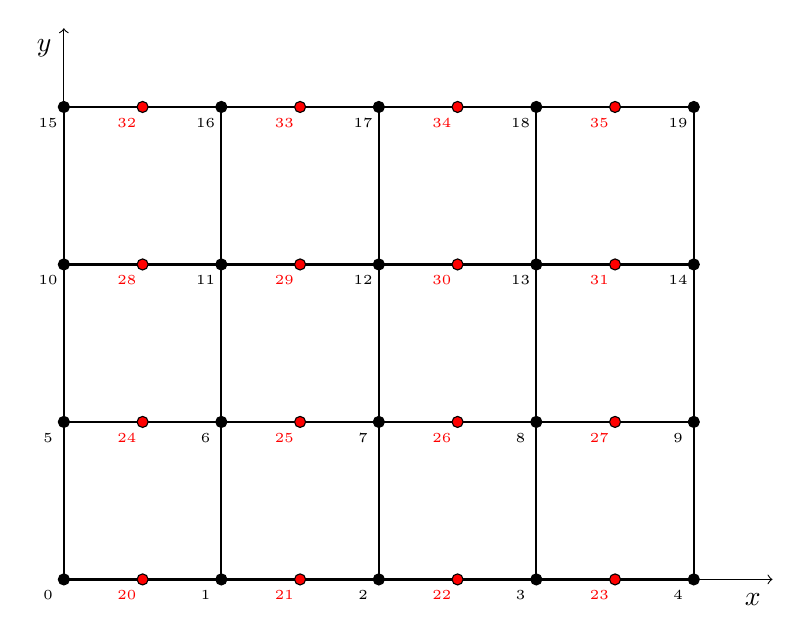
\begin{tikzpicture}
%\draw[fill=gray!23,gray!23](0,0) rectangle (10,8);
%\draw[step=0.5cm,gray,very thin] (0,0) grid (10,8); %background grid

\draw[thick] (1,1) -- (9,1) ;
\draw[thick] (1,3) -- (9,3) ;
\draw[thick] (1,5) -- (9,5) ;
\draw[thick] (1,7) -- (9,7) ;

\draw[thick] (1,1) -- (1,7) ;
\draw[thick] (3,1) -- (3,7) ;
\draw[thick] (5,1) -- (5,7) ;
\draw[thick] (7,1) -- (7,7) ;
\draw[thick] (9,1) -- (9,7) ;

\draw[black,fill=black] (1,1)   circle (2pt);
\draw[black,fill=black] (3,1)   circle (2pt);
\draw[black,fill=black] (5,1)   circle (2pt);
\draw[black,fill=black] (7,1)   circle (2pt);
\draw[black,fill=black] (9,1)   circle (2pt);

\draw[black,fill=black] (1,3)   circle (2pt);
\draw[black,fill=black] (3,3)   circle (2pt);
\draw[black,fill=black] (5,3)   circle (2pt);
\draw[black,fill=black] (7,3)   circle (2pt);
\draw[black,fill=black] (9,3)   circle (2pt);

\draw[black,fill=black] (1,5)   circle (2pt);
\draw[black,fill=black] (3,5)   circle (2pt);
\draw[black,fill=black] (5,5)   circle (2pt);
\draw[black,fill=black] (7,5)   circle (2pt);
\draw[black,fill=black] (9,5)   circle (2pt);

\draw[black,fill=black] (1,7)   circle (2pt);
\draw[black,fill=black] (3,7)   circle (2pt);
\draw[black,fill=black] (5,7)   circle (2pt);
\draw[black,fill=black] (7,7)   circle (2pt);
\draw[black,fill=black] (9,7)   circle (2pt);

\draw[black,fill=red] (2,1) circle (2pt); 
\draw[black,fill=red] (4,1) circle (2pt); 
\draw[black,fill=red] (6,1) circle (2pt); 
\draw[black,fill=red] (8,1) circle (2pt); 

\draw[black,fill=red] (2,3) circle (2pt); 
\draw[black,fill=red] (4,3) circle (2pt); 
\draw[black,fill=red] (6,3) circle (2pt); 
\draw[black,fill=red] (8,3) circle (2pt); 

\draw[black,fill=red] (2,5) circle (2pt); 
\draw[black,fill=red] (4,5) circle (2pt); 
\draw[black,fill=red] (6,5) circle (2pt); 
\draw[black,fill=red] (8,5) circle (2pt); 

\draw[black,fill=red] (2,7) circle (2pt); 
\draw[black,fill=red] (4,7) circle (2pt); 
\draw[black,fill=red] (6,7) circle (2pt); 
\draw[black,fill=red] (8,7) circle (2pt); 

\draw[thin,->] (9,1) -- (10,1); %x
\draw[thin,->] (1,7) -- (1,8); %y
\node[] at (9.75,0.75) {$x$};
\node[] at (0.75,7.75) {$y$};

\node[] at (0.8,0.8) {\tiny 0};
\node[] at (2.8,0.8) {\tiny 1};
\node[] at (4.8,0.8) {\tiny 2};
\node[] at (6.8,0.8) {\tiny 3};
\node[] at (8.8,0.8) {\tiny 4};
\node[] at (0.8,2.8) {\tiny 5};
\node[] at (2.8,2.8) {\tiny 6};
\node[] at (4.8,2.8) {\tiny 7};
\node[] at (6.8,2.8) {\tiny 8};
\node[] at (8.8,2.8) {\tiny 9};
\node[] at (0.8,4.8) {\tiny 10};
\node[] at (2.8,4.8) {\tiny 11};
\node[] at (4.8,4.8) {\tiny 12};
\node[] at (6.8,4.8) {\tiny 13};
\node[] at (8.8,4.8) {\tiny 14};
\node[] at (0.8,6.8) {\tiny 15};
\node[] at (2.8,6.8) {\tiny 16};
\node[] at (4.8,6.8) {\tiny 17};
\node[] at (6.8,6.8) {\tiny 18};
\node[] at (8.8,6.8) {\tiny 19};

\node[] at (1.8,0.8) {\tiny \color{red} 20};
\node[] at (3.8,0.8) {\tiny \color{red} 21};
\node[] at (5.8,0.8) {\tiny \color{red} 22};
\node[] at (7.8,0.8) {\tiny \color{red} 23};

\node[] at (1.8,2.8) {\tiny \color{red} 24};
\node[] at (3.8,2.8) {\tiny \color{red} 25};
\node[] at (5.8,2.8) {\tiny \color{red} 26};
\node[] at (7.8,2.8) {\tiny \color{red} 27};

\node[] at (1.8,4.8) {\tiny \color{red} 28};
\node[] at (3.8,4.8) {\tiny \color{red} 29};
\node[] at (5.8,4.8) {\tiny \color{red} 30};
\node[] at (7.8,4.8) {\tiny \color{red} 31};

\node[] at (1.8,6.8) {\tiny \color{red} 32};
\node[] at (3.8,6.8) {\tiny \color{red} 33};
\node[] at (5.8,6.8) {\tiny \color{red} 34};
\node[] at (7.8,6.8) {\tiny \color{red} 35};

\end{tikzpicture}
\end{center}








\input{python_codes/fieldstone_161/tikz_gridv}

For this mesh we have 

\begin{lstlisting}
nelx=4
nely=3
nnx=nelx+1
nny=nely+1
nel=nelx*nely (=12) 
Nu=nnx*nny+nelx*nny (=20+16=36)
Nv=nnx*nny+nnx*nely (=20+15=35)
\end{lstlisting}

The total number of velocity dofs is 
\begin{lstlisting}
NfemV=Nu+Nv (=36+35=71)
\end{lstlisting}

What makes this element pair rather awkward to implement is the fact that 
there are two connectivity arrays {\tt iconu} and {\tt iconv}, both of size $mV\times nel$, where 
$mV=6$ is the number of nodes linked to an element for each velocity component. 
\begin{itemize}
\item content of {\tt iconu}
\begin{verbatim}
elt udofs 
0 | [ 0  1  6  5 20 24]
1 | [ 1  2  7  6 21 25]
2 | [ 2  3  8  7 22 26]
3 | [ 3  4  9  8 23 27]
4 | [ 5  6 11 10 24 28]
5 | [ 6  7 12 11 25 29]
6 | [ 7  8 13 12 26 30]
7 | [ 8  9 14 13 27 31]
8 | [10 11 16 15 28 32]
9 | [11 12 17 16 29 33]
10 | [12 13 18 17 30 34]
11 | [13 14 19 18 31 35]
\end{verbatim}
\item content of {\tt iconv}
\begin{verbatim}
elt vdofs 
0 | [ 0  1  6  5 20 21]
1 | [ 1  2  7  6 21 22]
2 | [ 2  3  8  7 22 23]
3 | [ 3  4  9  8 23 24]
4 | [ 5  6 11 10 25 26]
5 | [ 6  7 12 11 26 27]
6 | [ 7  8 13 12 27 28]
7 | [ 8  9 14 13 28 29]
8 | [10 11 16 15 30 31]
9 | [11 12 17 16 31 32]
10 | [12 13 18 17 32 33]
11 | [13 14 19 18 33 34]
\end{verbatim}
\end{itemize}

Unlike many other codes in this book the global solution vector $\vec{\cal V}$ 
is organised as follows:
\[
\vec{\cal V} = ( u_1, u_2, ... u_{Nu}, v_1, v_2, ... v_{Nv})
\]

As mentioned in the articles\footnote{See also Section~\ref{MMM-ss:qqq_elt}}  
\begin{displayquote}
{\color{darkgray}
It is difficult to find a
local basis for $P_h$. But on the other side, it is the special interest of the method that
the space $P_h$ can be omitted in computation and the discrete solutions approximating
the pressure function in the Stokes equations can be obtained as byproducts, as we
shall see next.}
\end{displayquote}
so I will leave the pressure dofs alone for now, and will come back to it a bit later.

Remark 1: given the weird placement of nodes for u and v, it makes sense not to 
use an isoparameteric mapping, and instead choose a simple $Q_1$ mapping (this 
is not very important here since all elements are rectangles anyways).

Remark 2: the paper does not mention quadrature at all. 
I choose a 3x3 quadrature as for $Q_2\times Q_1$. 
Should I use a different quadrature for the div-div term?

Remark 3: the papers also do not mention 3D, nor non-rectangular elements. 

%%%%%%%%%%%%%%%%%%%%%%%%%%%%%%%%%%%%
\section*{Iterated penalty method}

Following \cite{zhan09,huzh11} we implement this method since

\begin{displayquote}
{\color{darkgray}
it is the special interest
of the divergence-free finite element method that the space $P_h$ can be omitted
in computation and the discrete solutions approximating the pressure function
in the Stokes equations can be obtained as byproducts, if an iterated penalty
method is adopted to solve system (2.5).}
\end{displayquote}

Also in \textcite{huzh11}:
\begin{displayquote}
{\color{darkgray}
We do enough iterated penalty iterations (cf. [25,30]) until the iterative error is smaller
than the truncation error each time.}
\end{displayquote}

In \textcite{zhan09} we find the following definition:
\begin{center}
\fbox{\includegraphics[width=12cm]{python_codes/fieldstone_161/images/iterpen}}
\end{center}

Let us then write the first steps of this algorithm\footnote{For personal reasons
and to establish a parallel with the penalty method, I replace $\alpha$ by $\lambda$.}.
\begin{itemize}
\item
For $n=1$:
\begin{eqnarray}
a({\bm u}_h^1,{\bm v}_h) + \lambda (\text{div}\; {\bm u}_h^1, \text{div}\; {\bm v}_h) 
&=& ({\bm f} , {\bm v}_h) - \text{div}\; \left( \lambda {\bm u}_h^0 , \text{div}\; {\bm v}_h \right) \nn\\
p_h^1 &=& - \text{div}\; [\lambda ( {\bm u}_h^0 + {\bm u}_h^1 )]
\end{eqnarray}
\item 
For $n=2$:
\begin{eqnarray}
a({\bm u}_h^2,{\bm v}_h) + \lambda (\text{div}\; {\bm u}_h^2, \text{div}\; {\bm v}_h) 
&=& ({\bm f} , {\bm v}_h) - \text{div}\; \left( \lambda ({\bm u}_h^0 +{\bm u}_h^1 ), \text{div}\; {\bm v}_h \right) \nn\\
p_h^2 &=& - \text{div}\; [\lambda ( {\bm u}_h^0 + {\bm u}_h^1 + {\bm u}_h^2)]
\end{eqnarray}
\end{itemize}

Concretely, we start with ${\bm u}_h^0={\bm 0}$ and we compute the pressure only when the 
iterations have converged, i.e. the inf norm of the difference between two consecutive 
velocity fields is less than a user chosen tolerance:
\begin{lstlisting}
xi_u=np.max(abs(u_prev-u))/np.max(abs(u))
xi_v=np.max(abs(v_prev-v))/np.max(abs(v))
if xi_u<tol and xi_v<tol:
   break
\end{lstlisting}
These values are written at every iteration in the {\tt conv.ascii} file.

Once the velocity field has been obtained the pressure is computed 
at each corner of each element ($Q_{-1}$ representation).
We will see that it is indeed discontinuous (but not everywhere?!).


\newpage
%==========================================
\section*{Grids and dofs}

In \textcite{huzh11} we find the following table:

\begin{center}
\includegraphics[width=10cm]{python_codes/fieldstone_161/images/dofs}
\end{center}

The authors state that ``The initial grid, level one grid, is simply one unit square''
so that the level 2 grid is a $2\times 2$ element grid:
\begin{verbatim}
+-------+-------+
|       |       |
|       |       |
|       |       |
+-------+-------+
|       |       |
|       |       |
|       |       |
+-------+-------+
\end{verbatim}
with the following velocity dofs:
\begin{verbatim}
u---u---u---u---u   v-------v-------v
|       |       |   |       |       |
|       |       |   v       v       v
|       |       |   |       |       |
u---u---u---u---u   v-------v-------v
|       |       |   |       |       |
|       |       |   v       v       v
|       |       |   |       |       |
u---u---u---u---u   v-------v-------v
\end{verbatim}
Since $u=v=0$ on all boundaries we replace the $u,v$ dofs by $\times$
to indicate that these are no longer degrees of freedom:
\begin{verbatim}
x---x---x---x---x   x-------x-------x
|       |       |   |       |       |
|       |       |   x       v       x
|       |       |   |       |       |
x---u---u---u---x   x-------v-------x
|       |       |   |       |       |
|       |       |   x       v       x
|       |       |   |       |       |
x---x---x---x---x   x-------x-------x
\end{verbatim}
and we indeed find $\text{dim}~V_h=6$. 

\newpage
Let us now turn to a level 3 grid, i.e. $4\times 4$ elements. 
The $u$ dofs are placed as follows:
\begin{verbatim}
u---u---u---u---u---u---u---u---u
|       |       |       |       |
|       |       |       |       |
|       |       |       |       |
u---u---u---u---u---u---u---u---u
|       |       |       |       |
|       |       |       |       |
|       |       |       |       |
u---u---u---u---u---u---u---u---u
|       |       |       |       |
|       |       |       |       |
|       |       |       |       |
u---u---u---u---u---u---u---u---u
|       |       |       |       |
|       |       |       |       |
|       |       |       |       |
u---u---u---u---u---u---u---u---u
\end{verbatim}
After boundary conditions are imposed:
\begin{verbatim}
x---x---x---x---x---x---x---x---x
|       |       |       |       |
|       |       |       |       |
|       |       |       |       |
x---u---u---u---u---u---u---u---x
|       |       |       |       |
|       |       |       |       |
|       |       |       |       |
x---u---u---u---u---u---u---u---x
|       |       |       |       |
|       |       |       |       |
|       |       |       |       |
x---u---u---u---u---u---u---u---x
|       |       |       |       |
|       |       |       |       |
|       |       |       |       |
x---x---x---x---x---x---x---x---x
\end{verbatim}
Only 21 $u$ are left, and we will find as many $v$ dofs, so in this case $\text{dim}(V_h)=21+21=42$,
in accordance with the table. 

Let us now turn to the pressure dofs. 
Warning: it is not as simple as the velocity dofs. 
In \textcite{huzh11} we read: ``we decrease the space $Q_1^{dc}$ 
for the pressure to $Q_1'$, by removing all spurious modes, i.e.,
eliminating one degree of freedom at each vertex. We have to emphasize
that the discrete pressure space is introduced for the analysis, but not in the
computation. By an iterated penalty method, we obtain the discrete solutions
for the pressure without coding the pressure element''
and in 
\textcite{zhan09}:
``
We note that, by choosing div($Q_{k+1,k}\times Q_{k,k+1}$) 
as the discrete finite element space for the pressure, the spurious
modes in discontinuous $Q_k$ space are filtered out automatically.
[...]
$P_h$ is a subspace of discontinuous, piecewise polynomials
of separate-degree $k$ or less. As singular vertices are present (see [15, 16]), 
$P_h$ is a proper subset of the discontinuous piecewise $Q_k$ 
polynomials. It is difficult to find a local basis for $P_h$.
[...]
We note that the spurious (checkerboard) modes, generated at each 
singular vertex (cf. (3.8)), in the discrete pressure space are filtered
out naturally.
''

In order to understand this and arrive at the correct number of pressure dofs
presented in the table above 
it is useful to look at this part of \textcite{huzh11}:

\begin{center}
\fbox{\includegraphics[width=12cm]{python_codes/fieldstone_161/images/pconstraints}}
\end{center}

We see that all nodes are subjected to a constraint. After the mesh is divided 
in $2\times 2$ macro-elements we see that there are 3 type of vertices: the corner ones, 
the mid-edge ones, and the interior ones. 
Let us start with the simplest case: a $2\times 2$ element mesh, i.e. a single macro element.
If the pressure field was a `true' $Q_{-1}$ field\footnote{
Same as $Q_1^{dc}$, but I prefer $Q_{-1}$ to remain consistent 
with the rest of the book.}, we would have 4 pdofs per element,
so $4\cdot 4=16$ pdofs in total:
\begin{verbatim}
+-------+-------+
|4     3|4     3|
|       |       |
|1     2|1     2|
+-------+-------+
|4     3|4     3|
|       |       |
|1     2|1     2|
+-------+-------+
\end{verbatim}
However it is clear from the Eq.~(3.7) above that the corner nodes are constrained to 0, so we
have 4 constraints, i.e. 4 pdofs removed. 
The same equation tells us that mid-edge vertices are constrained (i.e. the pressure 
is continuous at those vertices) so we have again 4 more constraints.
Finally there is one constraint for the vertex in the middle, and one should not 
forget that the pressure space is such that  $\int _\Omega p \; dV=0$, which 
introduces a last constraint. 
In total, 4+4+1+1=10 constraints, so we are left with 16-10=6 pdofs, which is the 
number in the table.

We also find in \textcite{zhmu16}\footnote{That paper is about a different 
FE pair, that is not divergence-free, but it presents the pressure space
of our FE element here.} a rewording of the constraints:
\begin{center}
\fbox{\includegraphics[width=14cm]{python_codes/fieldstone_161/images/zhmu16}}
\end{center}

Let us look at a $4\times 4$ element mesh, i.e. a $2\times 2$ macro element as in the figure above. 
\begin{verbatim}
C-------+-------+-------+-------C
|4     3|4     3|4     3|4     3|
|       |       |       |       |
|1     2|1     2|1     2|1     2|
+-------+-------+-------+-------+
|4     3|4     3|4     3|4     3|
|       |       |       |       |
|1     2|1     2|1     2|1     2|
+-------+-------+-------+-------+
|4     3|4     3|4     3|4     3|
|       |       |       |       |
|1     2|1     2|1     2|1     2|
+-------+-------+-------+-------+
|4     3|4     3|4     3|4     3|
|       |       |       |       |
|1     2|1     2|1     2|1     2|
C-------+-------+-------+-------C
\end{verbatim}
We start from potentially $16\cdot 4=64$ pdofs. We find that 
{\it all} vertices are subjected to a constraint, either because located on a 
corner, an edge or in the middle of four elements. 
This explains the sentence 
``we decrease the space $Q_1^{dc}$ for the pressure to $Q_1'$, by removing 
all spurious modes, i.e., eliminating one degree of freedom at each vertex.''
In the end each vertex is assigned a constraint, which removes as many 
pdofs. In this case, $5\cdot 5=25$ constraints. Taking into account the zero-average
constraint, we are left with 64-25-1=38 pdofs, as in the table!

Concretely if the mesh is composed of $n \times n$ elements, then it 
counts $4n^2 - (n+1)^2  -1$ pdofs.
\begin{itemize}
\item $n=2$:  $4n^2 - (n+1)^2 -1= 16 -9 -1=6 $ (we covered that already)
\item $n=4$:  $4n^2 - (n+1)^2 -1= 64 -25 -1=38 $ (we covered that already)
\item $n=8$:  $4n^2 - (n+1)^2 -1= 256 -81 -1=174 $ (value in the table)
\item $n=16$: $4n^2 - (n+1)^2 -1= 1024 -289 -1= 734$ (value in the table)
\end{itemize}

Having understood this, it is clear that it would be very difficult 
to come up with analytical expressions for the pressure basis functions. 

{\color{red} Q: what are the consequences of eq(3.7) (i.e. p=0 at corners?!) for 
generic cases?}

Remark: quid of odd numbers of elts (per side)? I have tried this, 
and in practice, this makes no difference in the error values nor their 
convergence rates.

%==========================================
\section*{Manufactured solutions}

\subsection*{Huang \& Zhang manufactured solution}

In \textcite{huzh11} (2011) the authors propose the 
following manufactured solution\footnote{I have removed the $2^8$ term.}:

\[
g(x,y)=(x-x^2)^2(y-y^2)^2 = 2^8 f(x)h(y) = 256 f(x) h(y)
\]
The velocity is given by 
\[
\vec\upnu 
= 
\left(
\begin{array}{c}
g_y \\ -g_x
\end{array}
\right)
=
\left(
\begin{array}{c}
256 fh' \\
-256 f'h
\end{array}
\right)
%=
%\left(
%\begin{array}{c}
%2^9(x-x^2)^2(1-2y)(y-y^2) \\
%-2^9(1-2x)(x-x^2)(y-y^2)^2 
%\end{array}
%\right)
\]
and the pressure is defined as
\[
p
= -g_{xx}
= -256 f'' h
\]
We have (assuming viscosity is 1) 
\[
\vec{f} = -\Delta \vec{\upnu} + \vec\nabla p
%= 
%\left(
%\begin{array}{c}
%- \Delta g_{y} -g_{xxx}\\
%- \Delta g_{x} -g_{yxx}
%\end{array}
%\right)
%= 
%\left(
%\begin{array}{c}
%- g_{yxx} - g_{yyy} -g_{xxx}\\
%  g_{xxx} + g_{xyy} -g_{yxx}
%\end{array}
%\right)
=256
\left(
\begin{array}{c}
- \Delta (fh') -f''' h  \\
-\Delta (-f'h) -f''h'
\end{array}
\right)
=256
\left(
\begin{array}{c}
- f''h' - fh''' -f''' h  \\
 f'''h + f'h''  -f''h'
\end{array}
\right)
\]
with
\begin{eqnarray}
f(x)&=& (x-x^2)^2 \nn\\
f'(x) &=& 2(1-2x)(x-x^2) \nn\\
f''(x) &=& 2(1-6x+6x^2) \nn\\
f'''(x) &=& 24x-12 \nn
\end{eqnarray}

We have 
\begin{eqnarray}
\iint_\Omega p(x,y) dxdy 
&=& -256 \int_{0}^{+1}\int_{0}^{+1} f''(x) h(y) dxdy \nn\\
&=& -256 \int_{0}^{+1} f''(x) dx \cdot \int_{0}^{+1}  h(y) dy \nn\\
&=& -256 \int_{0}^{+1} 2(1-6x+6x^2) dx \cdot \int_{0}^{+1}  (y-y^2)^2 dy \nn\\
&=& -256 \cdot 0 \cdot \frac{1}{30}  \nn\\ 
&=& 0
\end{eqnarray}
and the pressure is zero at all four corners:
\[
p(0,0)=p(1,1)=p(0,1)=p(1,0)=0
\]


\begin{center}
\fbox{\includegraphics[width=13cm]{python_codes/fieldstone_161/images/mms}}\\
{\captionfont Taken from \cite{zhan09}. Second component of velocity and pressure fields.}
\end{center}

\begin{center}
\includegraphics[width=5cm]{python_codes/fieldstone_161/results/bench2/th_u}
\includegraphics[width=5cm]{python_codes/fieldstone_161/results/bench2/th_v}\\
\includegraphics[width=5cm]{python_codes/fieldstone_161/results/bench2/th_vel}
\includegraphics[width=5cm]{python_codes/fieldstone_161/results/bench2/th_press}\\
{\captionfont Figures obtained with Paraview. Visualisation of the analytical solution. 
factor $2^8$ missing.}
\end{center}

They also report the following rates:

\begin{center}
\includegraphics[width=13cm]{python_codes/fieldstone_161/images/errors}
\end{center}

It is quite remarkable that the error convergence rates (in the $L_2$ norm)
are identical for both velocity and pressure. 

%-------------------------------------------------
\subsection*{Donea \& Huerta manufactured solution}

Taken from \cite{dohu03}. We consider a two-dimensional problem 
in the square domain $\Omega=[0,1]\times[0,1]$, which possesses a closed-form analytical 
solution. The fluid viscosity is $\eta=1$.
The velocity and pressure fields are given by:
\begin{eqnarray}
u(x,y) 
&=& x^2(1- x)^2 (2y - 6y^2 + 4y^3)  \nn\\
&=& x^2(1-x)^2 2y (1-3y+2y^2) \nonumber\\
&=& x^2(1-x)^2 2y (y-1)(2y-1) \nonumber\\
v(x,y) 
&=& -y^2 (1 - y)^2 (2x - 6x^2 + 4x^3) \nn\\
&=& -y^2 (1 - y)^2 2x (1-3x+2x^2) \nonumber\\
&=& -y^2 (1 - y)^2 2x (x-1)(2x-1) \nonumber\\
p(x,y) &=& x(1 -x)- 1/6 \nonumber 
\end{eqnarray}
Note that the pressure obeys $\int_{\Omega} p \; dV = 0$.

The components of the body force $\vec{b}$ are then
\begin{eqnarray}
b_x &=& (12 - 24y) x^4 + (-24 + 48y) x^3 + (-48y + 72y^2 - 48 y^3 + 12) x^2 \nonumber\\
    && + (-2 + 24y -72y^2+48y^3)x + 1-4y + 12y^2-8y^3 \nonumber\\ 
b_y &=& (8 - 48y + 48 y^2) x^3 + (-12 + 72y - 72y^2) x^2  \nonumber\\
    && + (4 - 24y + 48y^2 - 48y^3 + 24y^4) x - 12y^2 + 24y^3 - 12y^4  \nonumber
\end{eqnarray}

We find that the velocity fields are identical across 
both benchmarks. Only the pressure fields differ!

%=========================
\section*{code structure}

\begin{verbatim}
build mesh arrays, xu, yu, xv, yv
build connectivity arrays iconu, iconv
define boundary conditions
for iter in range(0,niter):
    build FE matrix and rhs
    solve linear system
    check convergence of u and v fields
compute Q_{-1} pressure and div(v)
compute int p dV
compute divv on markers
compute L2 errors v,p,div(v)
export to paraview
\end{verbatim}
The chosen format for the vtu file is $Q_{-1}$: each element
is exported separately, and 4 corner values for 
each $u$, $v$, $p$, $div(v)$ field.

The {\python bench} parameter allows to choose 
which benchmark is carried out.

All functions are jitted.

Because all elements are rectangles the mapping is trivial
and analytical. 

The following results are obtained by running the basch script
{\tt script\_errors}.

\newpage
%============================
\section*{Results}

Note that in what follows I use a direct solver as provided by scipy.

%------------------------------------------------------------
\subsection*{Donea \& Huerta manufactured solution ({\tt bench=1})}

\subsubsection*{Without iterations}

Let us first explore the influence of the $\lambda$ parameter:

\begin{center}
\includegraphics[width=5.7cm]{python_codes/fieldstone_161/results/bench1/single/errorsV.pdf}
\includegraphics[width=5.7cm]{python_codes/fieldstone_161/results/bench1/single/errorsP.pdf}
\end{center}

This is in essence a strong penalty problem, but the accuracy clearly decreases 
with increasing resolution. 

\subsubsection*{With iterations}

\begin{center}
\includegraphics[width=5.7cm]{python_codes/fieldstone_161/results/bench1/iterations/errorsV.pdf}
\includegraphics[width=5.7cm]{python_codes/fieldstone_161/results/bench1/iterations/errorsP.pdf}
\includegraphics[width=5.7cm]{python_codes/fieldstone_161/results/bench1/iterations/errorsDivv.pdf}
\end{center}

Rates are not what is expected from this element, since the authors report 
second-order error rate convergence for both velocity and pressure.
We fnd that the $L_2$ norm of div(v) is very low and the higher $\lambda$ the lower 
the divergence.

\begin{center}
\includegraphics[width=5.7cm]{python_codes/fieldstone_161/results/bench1/iterations/conv1.pdf}
\includegraphics[width=5.7cm]{python_codes/fieldstone_161/results/bench1/iterations/conv2.pdf}
\includegraphics[width=5.7cm]{python_codes/fieldstone_161/results/bench1/iterations/conv3.pdf}\\
\includegraphics[width=5.7cm]{python_codes/fieldstone_161/results/bench1/iterations/conv4.pdf}
\includegraphics[width=5.7cm]{python_codes/fieldstone_161/results/bench1/iterations/conv5.pdf}
\includegraphics[width=5.7cm]{python_codes/fieldstone_161/results/bench1/iterations/conv6.pdf}
\end{center}

We find that for $\lambda \ge 10^2$ the number of iterations becomes really small.
Also the number of iterations to reach convergence decreases when $\lambda$ increases. 
Any value higher than $10^4$ does not improve the convergence, and even worse
at high resolution $\lambda=10^6$ does not converge anymore. 

Let us set $nelx=nely=16$ and $\lambda=10^3$ and let us look at the error fields, 
i.e. $v_h-v$ and $p_h-p$:
\begin{center}
\includegraphics[width=5.7cm]{python_codes/fieldstone_161/results/bench1/iterations/press2}
\includegraphics[width=5.7cm]{python_codes/fieldstone_161/results/bench1/iterations/vel_error}
\includegraphics[width=5.7cm]{python_codes/fieldstone_161/results/bench1/iterations/press_error}\\
{\captionfont Left: pressure field; Middle: velocity error; Right: pressure error.} 
\end{center}
The analytical pressure field is $p(x,y)=x(1-x)-1/6$. The 1/6=0.16667 term insures that $\int p dV=0$.
We see that the constraints $p=0$ in the corners yield to an error that is exactly 1/6 there. 
Everywhere else the error is small, the continuity requirements on the edges do not interfere 
with the true solution. 
This is a huge problem that is not discussed in the original paper!




%------------------------------------------------------------ 
\subsection*{Huang \& Zhang manufactured solution ({\tt bench=2})}

\begin{center}
\includegraphics[width=8cm]{python_codes/fieldstone_161/results/bench2/errorsV.pdf}
\includegraphics[width=8cm]{python_codes/fieldstone_161/results/bench2/errorsP.pdf}\\
\end{center}

This time, we do recover second order convergence rate for pressure!
However there seems to be an exact factor 2 between my error and theirs.


\begin{center}
\includegraphics[width=5.7cm]{python_codes/fieldstone_161/results/bench2/conv1.pdf}
\includegraphics[width=5.7cm]{python_codes/fieldstone_161/results/bench2/conv2.pdf}
\includegraphics[width=5.7cm]{python_codes/fieldstone_161/results/bench2/conv3.pdf}\\
\includegraphics[width=5.7cm]{python_codes/fieldstone_161/results/bench2/conv4.pdf}
\includegraphics[width=5.7cm]{python_codes/fieldstone_161/results/bench2/conv5.pdf}
\includegraphics[width=5.7cm]{python_codes/fieldstone_161/results/bench2/conv6.pdf}
\end{center}

Note that at high resolution the case $\lambda=10^6$ fails to converge to the 
desired tolerance. 

\begin{center}
\includegraphics[width=5cm]{python_codes/fieldstone_161/results/bench2/press}
\includegraphics[width=5cm]{python_codes/fieldstone_161/results/bench2/press_error}
\includegraphics[width=5cm]{python_codes/fieldstone_161/results/bench2/press_error2}\\
\includegraphics[width=5cm]{python_codes/fieldstone_161/results/bench2/divv}
\includegraphics[width=5cm]{python_codes/fieldstone_161/results/bench2/vel_error}\\
{\captionfont Obtained on 8x8 grid (pressure was not x256 back then). 
We find that the divergence is indeed very low.
Note that Paraview is misleading: it looks like the squares are divived into 2 triangles but
in reality it is a visualisation artefact!}
\end{center}

It looks like pressure is continuous on the edges of the domain, 
which is indeed what we expect.


%----------------------------------
\section*{Conclusions}

\begin{itemize}

\item grid/vertex layout awkward to build. probably need re-ordering to 
get a matrix with reasonable skyline

\item pressure field is too complex to build so we have to use iterative penalty method. 
It seems to converge reasonably nice for $\lambda=10-100$ so this should not 
be too much of a pb for an iterative solver.

\item Q21-Q12 space smaller than than Q2xQ2 so A block smaller for a given number 
of elements. Also, the linear system is as big as the A-block, so in case one uses 
a direct solver, cheaper than solving matrix coming from mixed formulation

\item bonus: divergence free element!

\item with Q2Q1, we must iterate (outer solver to arrive at solution, FGMRES, or PCG. 
With this element, outer iterations also necessary. What is best?

\item quid of pressure not zero at corners? write Zhang ? try different mms 

\item matrix does not change during the iterations, this can be exploited!

\end{itemize}

